\documentclass[main.tex]{subfiles}
\pagestyle{main}

\begin{document}
\chapter{Exploration de différentes pénalisations sur la fonction coût utilisée pour optimiser les niveaux de gris \label{chap:anx_penalisation} }
\chaptermark{Exploration de différentes pénalisations} %%% Titre court pour l'entete
%\mylettrine{B}{labla}

\section{Régularisation de Moreau-Yosida}
\subsection{Présentation de la régularisation et propriétés}
\begin{dfn}\label{dfn:moreau_yosida}
Soit $J : \reel^n \longrightarrow \reel$ une fonction. La transformée (ou régularisée) de Moreau-Yosida de $J$ est définie à l'aide d'un paramètre $c>0$ par
\begin{equation}
J_c(u) := \min_{v\in \reel^n} \left( J(v) + \frac{1}{2c} \|v-u\|^2 \right).
\end{equation}
\end{dfn}
\noindent En prenant $v=u$ dans le minimum, on obtiens que~:
\begin{prop}
$\forall c>0, \quad \forall u \in \reel^n, \quad J_c(u) \leq J(u) .$
\end{prop}
\noindent Si $J$ est une fonction à minimiser, alors la propriété suivante est utile~:
\begin{prop}
Soit $a$ le minimum de $J$. Soit $u$ l'un des antécédants de $a$. Alors $u$ minimise aussi $J_c$ et on a $J_c(u)=J(u)=a$ quelque soit $c>0$.
\end{prop}
\begin{proof}Notons $f_u(v) := J(v) + \frac{1}{2c} \| v-u \|^2$.
\begin{myitemize}
\item[$\Rightarrow$)] Soit $u_0$, un point en lequel $J$ atteint son minimum. \\
On a alors $f_{u_0}(u_0) = J(u_0)\leq J(u) \leq J(u) + \frac{1}{2c} \| u-u_0 \|^2  = f_{u_0}(u), \ \forall u $, \\
d'où $J_c(u_0) = \min_u f_{u_0}(u) = J(u_0) $. On a donc égalité des fonctions $J$ et $J_c$ en $u_0$. Reste à montrer que $u_0$ est bien un point de minimum pour $J_c$. Comme $u_0$ minimise $J$, on a $J(u_0)\leq J(v), \ \forall v$. \\
d'où $ J(u_0) + \frac{1}{2c}\|v-u\|^2 \leq J(v) + \frac{1}{2c}\| v-u \|^2, \ \forall u, \forall v$.\\
Ainsi $ \min_v ( J(u_0) + \frac{1}{2c}\|v-u\|^2 ) \leq \min_v ( J(v) + \frac{1}{2c}\| v-u \|^2)=J_c(u) \ \forall u$. \\
Or $\min_v ( J(u_0) + \frac{1}{2c}\|v-u\|^2 )=J(u_0)$ et $J(u_0)=J_c(u_0)$\\ donc $J_c(u_0) \leq J(u), \ \forall u $.
et ainsi $u_0$ minimise $J_c$.
\item[$\Leftarrow$)] Supposons que $u_0$ minimise $J_c$. On a alors
\begin{center}
$J_c(u_0) \leq J_c(u) = \min_v f_u(v) \leq f_u(u) = J(u) \quad \forall u.$
\end{center}
Mais $J_c(u_0) = J(u_0)$. Ainsi $J(u_0) \leq J(u), \ \forall u$ 
et donc $u_0$ minimise $J$.
\end{myitemize}
\end{proof}
Ainsi minimiser la fonction $J$ est équivalent à minimiser la fonction $J_c$. 
L'avantage de la fonction $J_c$, c'est qu'elle est construite de sorte à être  différentiable aux abords du point de minimum même si $J$ ne l'est pas ($J$ peut même être discontinue). Le principal désavantage, c'est que le problème $\min_u J_c(u)$ est infiniment plus complexe à résoudre que le problème $\min_u J(u)$ puisque la fonction $J_c$ nécessite le calcul d'un minimum à chaque évaluation. Qu'à cela ne tienne. Dans notre cas, nous connaissons explicitement $J$. La transformée de Moreau-Yosida n'est appliquée que pour gagner en régularité. Ainsi, on peut calculer explicitement $J_c$. Avant de fournir un exemple, remarquons que 
\begin{prop}
Si la fonction $J$ est paire, alors sa régularisée $J_c$ l'est aussi.
\end{prop}
\begin{proof}
\begin{align*}
J_c(-u)  & = \min_{v\in \reel} \left( J(v) + \frac{1}{2c} \| v+u \|^2 \right) \\
& =\min_{s\in \reel} \left( J(-s) + \frac{1}{2c} \| -s+u \|^2 \right) \qquad \textrm{en posant } s=-v \\
& = \min_{s\in \reel} \left( J(s) + \frac{1}{2c} \|s-u \|^2 \right) = J_c(u) \qquad \textrm{( car $J$ et $\|.\|^2$ sont paires )}.
\end{align*}
\end{proof}

Ceci va nous permettre d'alléger les calculs. Regardons en exemple, le calcul de la régularisée d'une fonction créneau.

\begin{multicols}{2}
\paragraph{Exemple :} Considérons la fonction créneau :
$$J(u)= \left\{  \begin{aligned}
0 \quad & \textrm{si } u \in [-a;a], \\ 1 \quad & \textrm{sinon}. 
\end{aligned}   \right. $$
On pose $f_u(v) = J(v) + \sfrac{\| v-u \|^2}{2c}$.
On a $f'_u(v) = (v-u)/c, \ \forall u \in \reel \setminus \{ -a, a \}. $
En $\pm a$, la dérivée n'est pas définie. \\
Puisque $J$ est paire, nous pouvons limiter l'étude de sa régularisée aux $u$ positifs. La fonction étant dicontinue en $a$, il faut distinguer 2 cas~:
\begin{center}
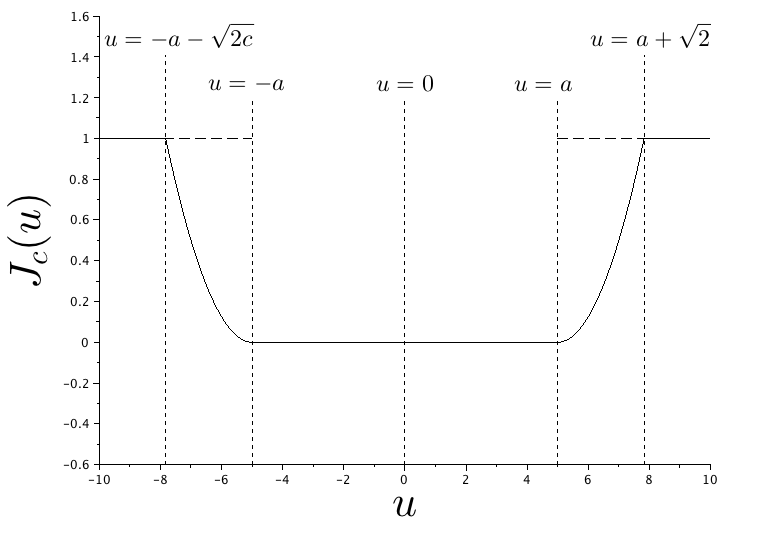
\includegraphics[width=.5\textwidth]{creneau.png}
\captionof{figure}{\label{fig:regul_creneau} Régularisation de Moreau-Yosida d'une fonction créneau avec~$c=4$. }
\end{center}
\end{multicols}
\begin{myitemize}
\renewcommand{\labelitemi}{\scriptsize$\bullet$} 
\item Cas 1 : $a < u$
\begin{center}
\begin{tikzpicture}
\tkzTabInit[espcl=2.8]{$v$/.7,$f_u'(v)$/.7,$f_u(v)$/1.7}{$0$, $a$, $u$, $+\infty$}
\tkzTabLine{,-,d,-,z,+}
\tkzTabVar{+/$\sfrac{u^2}{2c}$ , -CD+/$\sfrac{(a-u)^2}{2c}$/$ {\tiny 1+} \sfrac{(a-u)^2}{2c}$,-/$1$, +/$+\infty$ }
\end{tikzpicture}
\end{center}
Ici, $u\leq a \Rightarrow \min_v f_u(v) = \min \left(1, \sfrac{(a-u)^2}{2c} \right)  $. Ainsi $J_c$ vaut 1 si $\sfrac{(a-u)^2}{2c} \geq 1$, \ie si $u\leq a+\sqrt{2c}$; si $u>a+\sqrt{2c}$ alors $J_c(u)=\sfrac{(a-u)^2}{2c}$.
\item Cas 2 : $ a \geq u$. Ici tout les points $u$ tel que $0\leq u \leq a$ minimise $J$. Donc $J_c(u)=J(u)=0$ sur cet intervalle. On peut s'en rassurer avec le tableau de variation suivant~:
\begin{center}
\begin{tikzpicture}
\tkzTabInit[espcl=2.8]{$v$/.7,$f_u'(v)$/.7,$f_u(v)$/1.7}{$0$, $u$, $a$, $+\infty$}
\tkzTabLine{,-,z,-,d,+}
\tkzTabVar{+/$\sfrac{u^2}{2c}$,-/$0$,  +CD-/$\sfrac{(a-u)^2}{2c}$/$ {\tiny 1+} \sfrac{(a-u)^2}{2c}$, +/$+\infty$ }
\end{tikzpicture}
\end{center}
qui nous donne bien $J_c(u) = \min_v f_u(v) = 0$.
\end{myitemize}

\underline{Bilan :} On a une expression explicite de la régularisée (que l'on complète par parité de la fonction)~:
\begin{equation*}
J_c(u) = \left\{  \begin{aligned}
&1 && \textrm{ si } u\in ]-\infty;-a-\sqrt{2c}] \cup [a+\sqrt{2c};+\infty[  \\
&\sfrac{(a-u)^2}{2c} && \textrm{ si } u \in ]-a-\sqrt{2c};-a[ \cup ]a;a+\sqrt{2c} [ \\
&0 && \textrm{ si } u\in [-a;a]
\end{aligned}  \right.
\end{equation*}
L'allure de la fonction créneau~$J$ et de sa régularisée~$J_c$, sont présentées Figure~\ref{fig:regul_creneau}.

Notons que la fonction n'est régulière qu'aux abords des minimums. La valeur 0 est raccordé de manière dérivable, mais pas de dérivabilité pour le raccord en~$1$.

Remarquons également que plus le paramètre $c$ est grand, plus l'intervalle sur lequel agit la régularisation est large.


On pourrait aller beaucoup plus loin dans l'étude des propriétés de cette régularisation. De nombreuses publications ont été faite notament dans des cas où l'on ne connait pas analytiquement la fonction $J$ et où l'on s'intéresse notamment au problème adjoint... Nous ne nous étalerons pas plus sur ce vaste sujet : là n'est pas l'objet de ce manuscrit.

%%%%%%%%%%%%%%%%%
\subsection{Régularisation de Moreau-Yosida appliquée à une parabole tronquée.}
On considère dans cette section, la parabole tronquée suivante
\begin{equation}\label{eq:para_tronquee}
J(u) = [ u^2 - a^2 ]^+
\end{equation}
où $a^2$ est le minimum de la parabole d'origine, et où $[x]^+ = \max(x,0).$ De la même manière que dans l'exemple de la section précédente, nous allons construire explicitement la régularisée de cette fonction. On a ici~:
\begin{equation}
f_u(v) = [v^2-a^2]^+ + \frac{1}{2c}\|v-u\|^2.
\end{equation}
De plus, comme la fonction $J$ est paire, on restreint l'étude à l'ensemble $\reel_+$. Ainsi la dérivée est caractérisée sur $\reel_+$ par
\begin{equation}
f'_u(v) = \left\{  \begin{aligned}
&\frac{v-u}{c} && \textrm{ si } v<a,  \\
&\textrm{ non définie } && \textrm{ si } v=a, \\
& 2v+\frac{v-u}{c} && \textrm{ si } v>a.
\end{aligned}  \right.
\end{equation}
Ainsi
 \begin{equation} f'_u(v)=0
\Longleftrightarrow \left\{  \begin{aligned}
&v=u && \textrm{ si } v<a,  \\
& v=\frac{u}{2c+1} && \textrm{ si } v>a.
\end{aligned}  \right.
\end{equation}
Les cas suivants sont donc à considérer~(remarquer que comme $c>0$ et $u>0$ on a toujours $\frac{u}{2c+1}<u$):
\begin{myitemize}
\renewcommand{\labelitemi}{\scriptsize$\bullet$} 
\item Cas 1 : $0 < \frac{u}{2c+1} < u \leq a$\\ % \qquad$ 
%\raisebox{-20mm}{
%\begin{tikzpicture}
%\tkzTabInit[espcl=1.3]{$v$/.7,$f_u'(v)$/.7,$f_u(v)$/1}{$0$, $\frac{u}{2c+1}$ ,$u$, $a$, $+\infty$}
%\tkzTabLine{,-,,-,z,-,d,+}
%\tkzTabVar{+/ , R/ ,-/,  R/ , +/ }
%%%\tkzTabVal{1}{2}{0.5}{$\frac{u}{2c+1}$}{}
%\end{tikzpicture}}\\
%Ici, $\min_v f_u(v) = f(u) = [u^2-a^2]^+ = 0$
Dans ce cas là $u$ minimise $J$. Donc $J_c(u)=J(u)=0, \ \forall u \leq a$.

\item Cas 2 : $0 < \frac{u}{2c+1} < a < u \qquad$ 
\raisebox{-20mm}{
\begin{tikzpicture}
\tkzTabInit[espcl=1.3]{$v$/.7,$f_u'(v)$/.7,$f_u(v)$/1}{$0$, $\frac{u}{2c+1}$ ,$a$, $u$, $+\infty$}
\tkzTabLine{,-,,-,d,+,,+}
\tkzTabVar{+/ , R/ ,-/,  R/ , +/ }
%%\tkzTabVal{1}{2}{0.5}{$\frac{u}{2c+1}$}{}
\end{tikzpicture}}\\
Ici, $\min_v f_u(v) = f(a) = \frac{1}{2c} \| a-u\|^2, \ \forall u \in ]a,a(2c+1)[.$
\item Cas 2 : $0 < a < \frac{u}{2c+1} < u \qquad$ 
\raisebox{-20mm}{
\begin{tikzpicture}
\tkzTabInit[espcl=1.3]{$v$/.7,$f_u'(v)$/.7,$f_u(v)$/1}{$0$,$a$ , $\frac{u}{2c+1}$, $u$, $+\infty$}
\tkzTabLine{,-,d,-,z,+,,+}
\tkzTabVar{+/ , R/ ,-/,  R/ , +/ }
%%\tkzTabVal{1}{2}{0.5}{$\frac{u}{2c+1}$}{}
\end{tikzpicture}}\\
\begin{align*}
\textrm{Ici}, \min_v f_u(v) &= f\left( \frac{u}{2c+1} \right) = \left[ \left( \frac{u}{2c+1} \right)^2 -a^2 \right]^+ + \frac{1}{2c} \left\| \frac{u}{2c+1}-u \right\|^2 \\
& = \left( \frac{u}{2c+1} \right)^2 -a^2 + \frac{1}{2c} \left( \frac{-2cu}{2c+1} \right)^2 \\
& = \frac{u^2}{2c+1} -a^2, \quad \forall u \in ]a(2c+1),+\infty[.
\end{align*}
\end{myitemize}
\begin{figure}
\centering
\subfloat[\label{fig:para_tronquee} Parabole tronquée \newline $J(u)=$  {$[ u^2-a^2 ]^+ $} (avec $a=127.5$).]{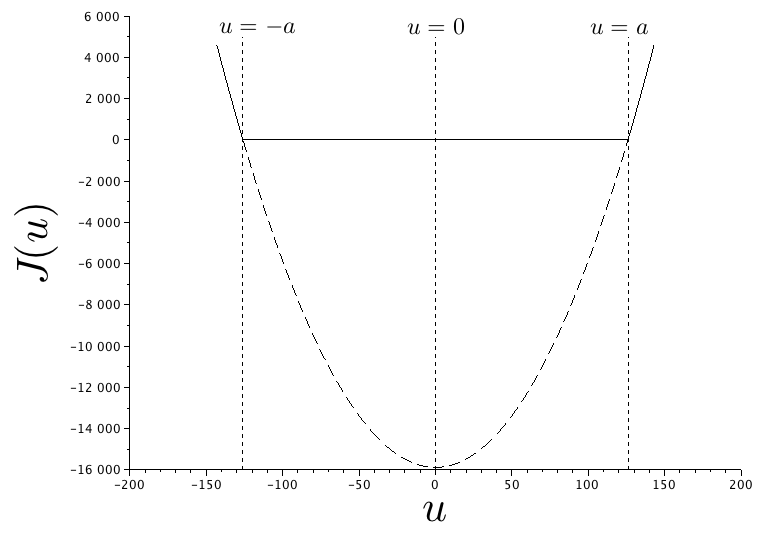
\includegraphics[width=.49\textwidth]{penal_quad.png}} 
\subfloat[\label{fig:regul_para_coupee} Régularisée de Moreau-Yosida d'une parabole tronquée ($c=0.1$).]{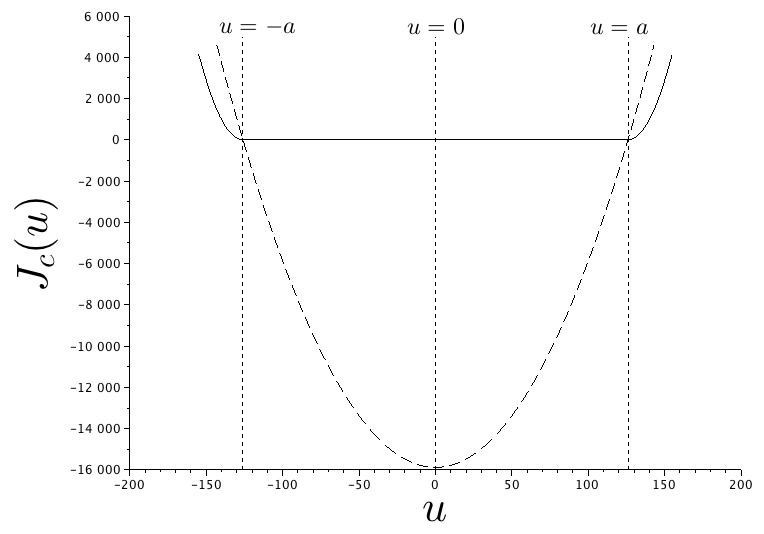
\includegraphics[width=.49\textwidth]{penal_quad_regul.png}}
\caption{\label{fig:regul_yosida} Exemple d'une régularisation de Moreau-Yosida.}
\end{figure}
Ainsi l'expression de la régularisée de la parabole tronquée~\ref{eq:para_tronquee} est donnée par
\begin{equation}\label{eq:regul_parabole_coupee}
J_c(u) = \left\{  \begin{aligned}
&\frac{u^2}{1+2c}-a^2 && \textrm{ si } u\in ]-\infty;-a(2c+1)] \cup [a(2c+1);+\infty[  \\
&\frac{1}{2c}\|a-u\|^2 && \textrm{ si } u \in ]-a(2c+1);-a[ \cup ]a;a(2c+1) [ \\
&0 && \textrm{ si } u\in [-a;a],
\end{aligned}  \right.
\end{equation}
et son allure est présentée sur la Figure~\ref{fig:regul_para_coupee}.

%%%%%%%%%%%
%%%%%%%%%%%
%%%%%%%%%%%
\section{Impact du choix de la pénalisation sur l'optimisation des niveaux de gris} %~: essais de diverses pénalisations sur la fonction coût}

%%%%%% Cout2
\DTLloaddb{optim2_2grey}{../data/cout_2_bad/optim2.csv}
\DTLloaddb[noheader]{optim2_2leg}{../data/cout_2_bad/optim2_leg.csv}
\DTLloaddb{optim2_2stat}{../data/cout_2_bad/optim2_stat.csv}
\DTLsetheader{optim2_2leg}{Column1}{}
\DTLsetheader{optim2_2leg}{Column2}{}
\begin{table}[htbp]
\footnotesize
\centering
\hspace{\retraittableau} %%% Le tableau depasse sur les marges !
\begin{tabular}{|c|c|c|c|c|}
\hline
\rowcolor{gray!70}
& \multicolumn{4}{c|}{ \cellcolor{gray!70} \bfseries  Algorithme d'optimisation} \\
\hhline{|>{\arrayrulecolor{gray!70}}->{\arrayrulecolor{black}}|-|-|-|-|}
\rowcolor{gray!70}
& \bfseries SLSQP
& \bfseries GC 
& \bfseries Neldear-Mead 
& \bfseries BFGS \\
\rowcolor{gray!70}
\multirow{-3}{\firstcolwidth}{\scriptsize \bfseries \centering Scanners choisis pour l'optimisation}
& $\tau_N, \qquad \tau_P$
& $\tau_N, \qquad \tau_P$
& $\tau_N, \qquad \tau_P$
& $\tau_N, \qquad \tau_P$
\DTLforeach*{optim2_2grey}{%
\scan=scan,\NM=NM,\BFGS=BFGS,\col=SLSQP,\CG=CG,
\errNM=errNM,\errBFGS=errBFGS,\errcol=errSLSQP,\errCG=errCG}{%
\\
\DTLifoddrow{\rowcolor{white}}{\rowcolor{gray!40}}%
\scan & \begin{tabular}{c}
\col \\ Err : \errcol
\end{tabular} & \begin{tabular}{c}
\CG \\ Err : \errCG
\end{tabular} & \begin{tabular}{c}
\NM \\ Err : \errNM
\end{tabular} & \begin{tabular}{c}
\BFGS \\Err : \errBFGS
\end{tabular} 
}%
%\DTLforeach*{optim2_2stat}{%
%\NM=NM,\BFGS=BFGS,\col=SLSQP,\CG=CG}{%
%\\ \hline \hline %\DTLifoddrow{\rowcolor{white}}{\rowcolor{gray!40}}%
%Moyenne : & \col & \CG & \NM & \BFGS  }
%\\ \hline
\end{tabular}

\caption{\label{tab:optim2gris_pen_quad}Tableau récapitulatif des optimisations réalisées sur 2 niveaux de gris, $\tau_S$ fixé à 197, avec pénalisation quadratique \eqref{eq:penalisation_quad} (\cf Figure~\ref{fig:para_tronquee}), pour les combinaisons défavorables de la Table~\ref{tab:optim2gris_bad}, page~\pageref{tab:optim2gris_bad}.}
\end{table}

Comme montré dans le chapitre \ref{chap:optim_grey} (\cf notamment Table~\ref{tab:optim2gris} et surtout dans la Table~\ref{tab:optim2gris_bad} ), les algorithmes d'optimisations sur les niveaux de gris tendent, dans certaines configurations,  vers des jeux de paramètres optimaux qui s'approchent du bord~0 ou du bord~255, voire même qui sont négatifs (\ie non convergence de l'algorithme d'optimisation). Ce phénomène pourrait être dû notamment au fait que la pénalisation en créneau \eqref{eq:penalisation_creneau} présente une discontinuité. Les algorithmes de descente notamment fonctionnant sur une approximation du gradient peuvent ainsi être perturbé par cette discontinuité. Examinons ceci de plus près. Essayons une pénalisation continue~: une parabole coupée
\begin{equation}
\label{eq:penalisation_quad}
\mathcal{P}(\tau) = \Big[ \big(  E(\tau) - 127.5 \big)^2-126^2 \Big]^+,
\end{equation}
où $[.]^+=\max(0,.)$ désigne la partie positive et où $E(\tau)$ est la composante de $\tau$ la plus éloignée du centre de l'intervalle autorisé (127.5 milieu de [0;255]):
\begin{equation}
\label{eq:tau_eloigne} E(\tau)= \arg\max_{i=1,2,3}( | \tau_i-127.5 | ).
\end{equation} 
L'aspect de cette pénalisation est présenté sur la Figure~\ref{fig:para_tronquee} (avec~$a=126; u=E(\tau)-127.5$). Il s'agit d'une parabole dont on ignore la partie négative. 
Ici la pénalisation intervient sur un intervalle légèrement plus court que~$[0;255]$, car de toute façon les valeurs de~$\tau$ n'ont pas à s'approcher de ces bornes (la pénalisation est non nulle en dehors de~$[1.5;253.5]$).



%\begin{figure}
%\centering
%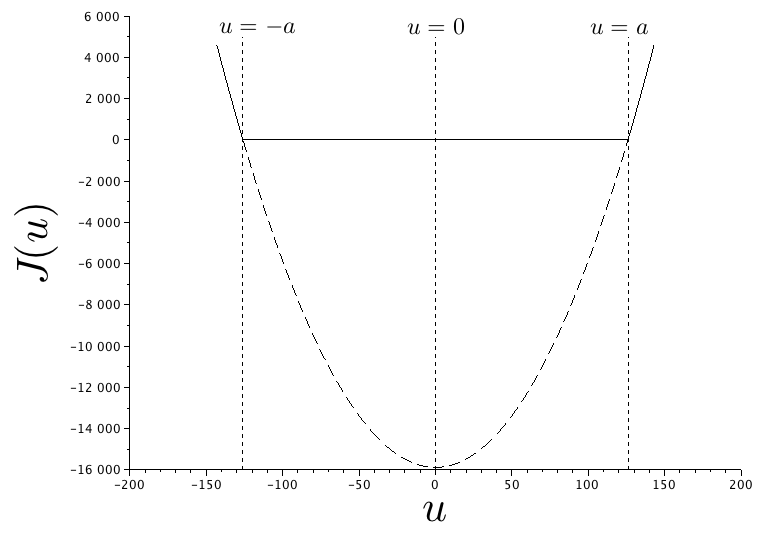
\includegraphics[width=.75\textwidth]{penal_quad.png}
%\vspace{-3mm}
%\caption{\label{fig:penal_quad} Pénalisation via une parabole tronquée (\cf Eq.~\eqref{eq:penalisation_quad}). }
%\end{figure}
Les résultats des optimisations de niveaux de gris faites avec la pénalisation~\eqref{eq:penalisation_quad} sont présentés dans la Table~\ref{tab:optim2gris_pen_quad}. Ici plus de valeurs négatives, cependant la borne 1.5 est atteinte à plusieurs reprises. De même les résultats entre les algorithmes sont très variables. Ainsi, ici, il est difficile de dire s'il y a eu une amélioration ou non par rapport à la pénalisation en créneau. 
La pénalisation considérée ici n'est que~$\mathcal{C}^0$ car il y a 2 points anguleux. Peut-être que cette régularité n'est pas suffisante encore.


%%%%%% Cout3
\DTLloaddb{optim2_grey}{../data/cout_3_bad/optim2.csv}
\DTLloaddb[noheader]{optim2_leg}{../data/cout_3_bad/optim2_leg.csv}
\DTLloaddb{optim2_stat}{../data/cout_3_bad/optim2_stat.csv}
\DTLsetheader{optim2_leg}{Column1}{}
\DTLsetheader{optim2_leg}{Column2}{}
\begin{table}[htpb]
\footnotesize
\centering
%\scriptsize
\hspace{\retraittableau} %%% Le tableau depasse sur les marges !
\begin{tabular}{|c|c|c|c|c|}
\hline
\rowcolor{gray!70}
& \multicolumn{4}{c|}{ \cellcolor{gray!70} \bfseries  Algorithme d'optimisation} \\
\hhline{|>{\arrayrulecolor{gray!70}}->{\arrayrulecolor{black}}|-|-|-|-|}
\rowcolor{gray!70}
& \bfseries SLSQP
& \bfseries GC 
& \bfseries Neldear-Mead 
& \bfseries BFGS \\
\rowcolor{gray!70}
\multirow{-3}{\firstcolwidth}{\scriptsize \bfseries \centering Scanners choisis pour l'optimisation}
& $\tau_N, \qquad \tau_P$
& $\tau_N, \qquad \tau_P$
& $\tau_N, \qquad \tau_P$
& $\tau_N, \qquad \tau_P$
\DTLforeach*{optim2_grey}{%
\scan=scan,\NM=NM,\BFGS=BFGS,\col=SLSQP,\CG=CG,
\errNM=errNM,\errBFGS=errBFGS,\errcol=errSLSQP,\errCG=errCG}{%
\\
\DTLifoddrow{\rowcolor{white}}{\rowcolor{gray!40}}%
\scan & \begin{tabular}{c}
\col \\ Err : \errcol
\end{tabular} & \begin{tabular}{c}
\CG \\ Err : \errCG
\end{tabular} & \begin{tabular}{c}
\NM \\ Err : \errNM
\end{tabular} & \begin{tabular}{c}
\BFGS \\ Err : \errBFGS
\end{tabular} 
}%
%\DTLforeach*{optim2_stat}{%
%\NM=NM,\BFGS=BFGS,\col=SLSQP,\CG=CG}{%
%\\ \hline \hline %\DTLifoddrow{\rowcolor{white}}{\rowcolor{gray!40}}%
%Moyenne : & \col & \CG & \NM & \BFGS  }
%\\ \hline
\end{tabular}
\caption{\label{tab:optim2gris_pen_quad_reg}Tableau récapitulatif des optimisations réalisées sur 2 niveaux de gris, $\tau_S$ fixé à 197, avec pour pénalisation une parabole tronquée régularisée (\cf Figure~\ref{fig:regul_para_coupee}), pour les configurations défavorables de la Table~\ref{tab:optim2gris_bad}, page~\pageref{tab:optim2gris_bad}.}
\end{table}
\todo{ref fig}

\DTLcleardb{optim2_leg}
\DTLcleardb{optim2_stat}
\DTLcleardb{optim2_grey}

Essayons donc une troisième fonction de pénalisation qui soit~$\mathcal{C}^1$. Considérons la régularisation de Moreau-Yosida de la pénalisation précédente. La courbe de la régularisée d'une parabole tronquée est représentée sur la Figure~\ref{fig:regul_para_coupee} (on prend ici $a=126; u=E(\tau)-127.5$). Les niveaux de gris optimaux obtenus avec cette nouvelle pénalisation plus régulière sont présentés dans la Table~\ref{tab:optim2gris_pen_quad_reg}.


Visiblement rien ne semble y faire : il y a toujours des valeurs de~$\tau_N$ qui s'approchent des bornes autorisées et les cas où l'on considère les images~$[2,5,7]$ et~$[3,7,9]$ par exemple  fournissent des résultats très différents selon les algorithmes d'optimisation utilisés, qui de plus font apparaître~$\tau_N$>>$\tau_S$ ce qui est aberrant.
La régularité de la pénalisation ne semblent donc pas en cause ici. Le problème semble donc venir d'ailleurs (\cf fin de la section~\ref{sec:optim_2_param} traitant des problèmes de mauvais  conditionnement de nos systèmes).

%En ce qui concerne l'aberration, cela peut venir du fait que les images 5,7 et 9 sont petites, et donc le bruit est très important et l'image numéro 3, de taille moyenne n'arrive pas à rattraper ce bruit. Il faut donc éviter de prendre en compte les images où la tumeur est trop petite, et si l'on en prend il faut que ces images soient minoritaires devant les autres.

\end{document}